\section{METHODS}\label{sec:methods}
\subsection{Digital Phantom}\label{sec:phantom}
Based on the fiber geometries of the digital phantom created
  for the \emph{\acrshort*{hardi} Reconstruction Challenge} held
  in ISBI 2013 (San Francisco, US), we simulated high resolution
  (0.5mm isotropic) T1 weighted (TE/TR= 10/1500ms) and T2w
  (TE/TR= 90/5000ms) images, as well as two \gls*{dmri} images
  (1.0mm isotropic, $b$=1200, 1 \emph{b0} image) with 32 and 64
  evenly-distributed directions intended for \gls*{dti} and 
  \gls*{hardi} reconstructions, respectively.
Diffusion is modeled by a restricted and a hindered compartment,
  similar to \cite{assaf_composite_2005}.
The phantom includes \gls*{wm} fiber bundles, \gls*{gm} and \gls*{csf}.
Physical properties (T1/T2 times in ms) used in simulation are
  ($832\pm10/79\pm0.6$) for \gls*{wm},
  ($1331\pm13/110\pm2.0$) for \gls*{gm} and
  ($3500\pm100$ / $250\pm10$) for \gls*{csf}.
T1w, T2w and \glspl*{dwi} were added normally distributed noise
  up to a \gls*{snr} of 30dB.

\subsection{Theory-based synthetic distortion}
\label{sec:distortion}
\Gls*{fmb} methodologies use a map of the field in the scanner.
More precisely, the phase difference between two subsequent samplings
  of the field map.
With that information, it is possible to compute the theoretical
  displacement that each voxel undergoes, the so-called \gls*{vsm}.
The most prominent feature of this \gls*{vsm} is that all the shifts
  have the same orientation (parallel to the phase-encoding direction
  of the \gls*{epi}) and their magnitude and direction depend on the 
  \gls*{epi} gradient increments (or \emph{blips})
  and the actual phase difference at the voxel.

In order to create a realistic distortion, we generated a synthetic and noise-free
  phase-difference map consistent with the phantom, using the tools distributed with
  the \emph{FSL} package %\cite{jenkinson_fsl_2012}
  (\url{www.fmrib.ox.ac.uk/fsl}) and standard parameters ($\Delta$TE=2.46~ms. for the
  field mapping and \emph{effective dwell time} of 0.77~ms for the \gls*{dwi}).
We defined two regions of smooth dephasing and computed the corresponding \gls*{vsm}.
Amplitude of the dephasing maps can be modulated, enabling us to evaluate the
  magnitude of distortion.
We generated several \glspl*{vsm} with increasing maximum shifts (from 3.80 to 7.60~mm),
  covering the typical magnitudes of distortion observed in real datasets.

From these synthetic \glspl*{vsm}, we generated the corresponding distorted \glspl*{dwi},
  in two opposed phase-gradient encoding directions.
The second simulated ``acquisition'' of the same phantom was necessary for evaluating \gls*{reb}
  methods.

In summary, we generated a full gold-standard containing realistic T1w and T2w
  at high resolution, \glspl*{dwi} acquired in two different phase encoding directions,
  and a ground-truth \gls*{dwi} data, which is not available for real datasets
  (\autoref{fig:phantom}).
%The dataset is completed with two more images, the noise-free field map used for
%  generating the \gls*{vsm} and a field map with normally distributed noise for
%  a \gls*{snr} of 20dB.


\begin{figure}[thpb]
   \centering
   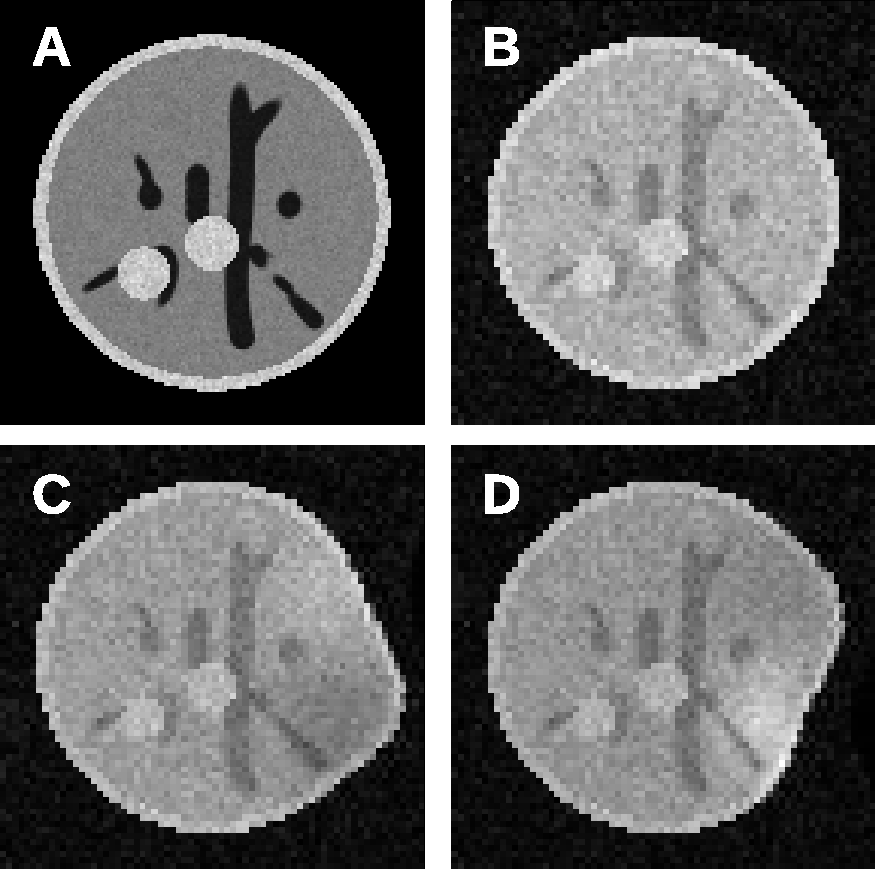
\includegraphics[width=0.95\columnwidth]{Fig01-Phantom}
   \caption{Ground-truth digital phantom.
   A) T2w; B) undistorted \textit{b0} volume;
   C, D) distorted \textit{b0} volumes with opposed phase 
   encoding directions, maximum displacement of 3.80~mm.}
   \label{fig:phantom}
\end{figure}

\subsection{Correction methods}
\label{sec:correction}
Three out of four methods presented in \autoref{sec:intro} were tested on the
  evaluation framework.
\Gls*{fmb} correction is the same as the one used for generating the distortion,
  working on the opposite direction.
Normally distributed noise was added to the synthetic field map (\gls*{snr}=20dB)
  before correction, for a more realistic evaluation.
\Gls*{reb} correction is implemented in \emph{FSL} (\texttt{topup}), and it demands for the \textit{b0}
  of the reverse-encoding simulation.
In this second case, the \gls*{vsm} is inferred from the differences between the two corresponding 
  \textit{b0}.
Finally, we included \Gls*{t2b} methods with \emph{ANTs} (\url{stnava.github.io/ANTs}),
  fine-tuned for \textit{b0}-to-T2w registration.
To this end, we used a multi-resolution scheme with 3 levels of subsampling and smoothing,
  mutual information metric, and the symmetric diffeomorphic transform model.
Several configurations of kernel widths for the regularization smoothers were tested, and finally
  selected 0.5/1.0 voxels (gradient/deformation fields, respectively) for its best result.
Additionally, undistorted images are corrected for dropout using the determinant of the Jacobian 
  of the deformation field.

\subsection{Evaluation}
\label{sec:evaluation}
The original phantom, one distorted version, and the corrected instances are then connected to a
  \gls*{dwi} reconstruction and tractography pipeline.
Additionally, the original tissue probability maps are also distorted and corrected to provide
  tractography with the required \gls*{wm} masks.
These maps are also used in a final assessment module.

The framework supports two different methods for \gls*{dwi} reconstruction and deterministic
  tractography:
1) \emph{Diffusion Toolkit} (\url{trackvis.org/dtk}) %\cite{wang_diffusion_2007}
  for \gls*{dti}, is configured with 10 random seeds per voxel by default; and
2) \emph{MRTrix} %\cite{tournier_mrtrix:_2012}
  (\url{www.brain.org.au/software/mrtrix}) for \gls*{hardi}, with default parameters
  set to use constrained spherical deconvolution, maximum harmonic order of 6, and
  150000 desired tracks.
For both options, the seeding regions can be set to use either the distorted-corrected 
  \gls*{wm} mask, or the regions used to generate the ground-truth.
This second seeding strategy mimics the usual procedure on real data,
  where regions are typically mapped from the anatomically correct T1w.

The evaluation framework is completed by automated assessment modules.
We evaluated three characteristics of the correction methods.
Firstly, we assessed the geometrical correctness reporting overlap indices of three tissue
  probability maps (namely \gls*{csf}, \gls*{wm}, and \gls*{gm}), weighting the average by
  tissue volumes.
Secondly, to evaluate the quality of the actual signal dropout correction, we studied the 
  similarity volume by volume computing the $\ell_1$-norm correlation index.
We report this score on the \textit{b0} and the average of the remaining \gls*{dwi} volumes.
Thirdly, we studied the impact on the connectivity matrices reporting the number of 
  false positives (nonexistent connections in the gold-standard) and false negatives 
  (or missed connections).